\scanpage{55}

\uline{Corollaire} Les types numériques possibles de syst. de Schwartz pour $H=\mathrm{Aut}^{+}(\Pi)$ sont les suivants

\[
\begin{aligned}
\text{a)}\ &(4,3,2)\ (3,2,4)\ (2,4,3)\ (2,3,4)\ (3,4,2)\ (4,2,3)\\
&\hspace{18em}\text{(canoniques)}\\
\text{b)}\ &(4,4,3)\ (4,3,4)\ (3,4,4)
\end{aligned}
\]

Le type numérique détermine le syst. de Schwartz modulo conjugaison. De façon précise, si $\Sigma=(\rho,\rho',\rho'')$ est un syst. de Schwartz, alors \unsure{elle|on|il} est dans l'un ou l'autre des cas suivants, s'excluant mutuellement

a) $\unsure{\exists\!\mid|\exists!|\exists}$ repère direct $r\in R^{+}$ \inserted{(unique)} tel que $\Sigma$ soit égal à $\Sigma_r$ ou un de ses transformé par $\sigma\in\unsure{\mathfrak S_3|\mathcal S_3}$ ($\sigma$ unique aussi)

b) $\exists\!\mid$ \deleted{arc \unsure{$s,t,f$}} $r\in R^{+}$, $r=(s,\{s,\deleted{\unsure{s'}}t\},f)$, \deleted{et} tel que $\Sigma$ soit égal à $(\rho_s,\rho_t,\rho_f)$ ou à un transformé par $\sigma\in\mathfrak S_3^{+}$ ($\sigma$ aussi unique).

\figure{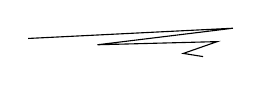
\begin{tikzpicture}\draw(0,0)--(2.6,.13)--(.88,-.08)--(2.4,-.04)--(1.97,-.19)--(2.22,-.23);\end{tikzpicture}}

Dém de d). Les ordres des él. $\ne1$ de $H$ sont $2,3,4$. Montrons d'abord qu'un système de Schwartz contient au moins un él. d'ordre $4$, et un \unsure{él|él.} d'ordre $3$.

% archive sheet number: 54
